\documentclass[main.tex]{subfiles}

\begin{document}

\section*{Goal}
Today we will examine the force that causes an object to follow a circular path. In our first experiment, we will create a centripetal force by whirling around at constant angular velocity an object attached to a spring. We will compare this centripetal force to the force needed to stretch the spring itself. In our second experiment, we will plot the centripetal force on a pendulum bob using a Force Sensor then compare it to the force that we will calculate from the speed of the pendulum as measured by a Photogate.

\section*{Equipment}
\begin{itemize}
\item
850 Universal Interface
\item
PASCO Capstone Software
\item
Centripetal Force Apparatus
\item
Masses and mass hanger
\item
Meter Stick
\item
Timer
\item
Triple-beam Balance
\item
Force Sensor and Photogate
\item
Lab post, rod and clamps for Force Sensor
\item
Pendulum bob and string
\end{itemize}•

\section*{Theory}
In order to have an object follow a curved path we need to have an acceleration towards the center of the circle. We call this center-seeking acceleration a centripetal acceleration. The magnitude is given by,
\begin{equation}\label{eq:CenAcc}
a_{c}=\frac{v^2}{r}.
\end{equation}
Let's quickly prove this. We know that an acceleration is defined as a change in velocity,
\begin{equation}\label{eq:Acc}
\mathbf{a} = \frac{\Delta \mathbf{v}}{\Delta t} = \frac{\mathbf{v}_f-\mathbf{v}_i}{t_f-t_i}.
\end{equation}

\begin{wrapfigure}{r}{0.5\textwidth}
\centering
\begin{subfigure}[h]{0.5\textwidth}
\centering
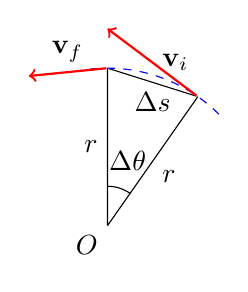
\begin{tikzpicture}
\draw (2,1) node[below left] {$O$} -- ++(55:2cm) node[outer sep = 0pt, inner sep = 0pt] (A) {} node [midway, below right] {$r$}
	 (2,1) -- ++(90:2cm) node[outer sep = 0pt, inner sep = 0pt] (B) {} node [midway, left] {$r$};
\draw (A) -- (B) node [midway, below] {$\Delta s$};

\draw[dashed,blue] ([shift=(45:2cm)] 2,1) arc (45:100:2cm);
\draw ([shift=(55:0.5cm)] 2,1) arc (55:90:0.5cm) node [above, xshift=2pt] at ([shift=(72:0.6cm)] 2,1) {$\Delta\theta$};

\draw[->,thick,red] (A) -- (2,3.5) node[midway, right, black] {$\mathbf{v}_i$};
\draw[->,thick,red] (B) -- (1,2.9) node[midway, above, black] {$\mathbf{v}_f$};
\end{tikzpicture}
\caption{} \label{fig:pos}
\end{subfigure}

\begin{subfigure}[h]{0.5\textwidth}
\centering
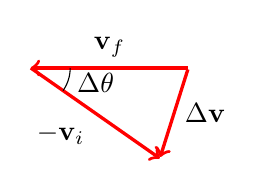
\begin{tikzpicture}
\draw[->,very thick,red,rotate=-90] (2,1) -- ++(55:2cm) node[outer sep = 0pt, inner sep = 0pt] (A) {} node [midway, below left, black] {$-\mathbf{v}_i$};
\draw[<-,very thick,red,rotate=-90] (2,1) -- ++(90:2cm) node[outer sep = 0pt, inner sep = 0pt] (B) {} node [midway, above, black] {$\mathbf{v}_f$};
\draw[->,very thick,red] (B) -- (A) node[midway, right, black] {$\Delta\mathbf{v}$};

\draw[rotate=-90] ([shift=(55:0.5cm)] 2,1) arc (55:90:0.5cm) node [right, xshift=-3pt] at ([shift=(72:0.6cm)] 2,1) {$\Delta\theta$};
\end{tikzpicture}
\caption{} \label{fig:vel}
\end{subfigure}
\caption{}
\vspace{-10pt}
\end{wrapfigure}

As the triangle in Figure~\ref{fig:pos} is similar to the triangle in Figure~\ref{fig:vel} the ratios of their sides will be equal,
\[
\frac{\Delta v}{v}=\frac{\Delta s}{r}.
\]
Therefore we can solve for $\Delta v,$
\begin{equation}\label{eq:DeltaV}
\Delta v = \frac{\Delta s}{r}v.
\end{equation}
But $\Delta s = v \Delta t$ so if we substitute this and Equation~\eqref{eq:DeltaV} into~\eqref{eq:Acc} we have,
\[
a_c =\frac{\Delta v}{\Delta t}=\frac{\Delta s}{\Delta t}\frac{v}{r}=\frac{v^2}{r},
\]
which is exactly Equation~\eqref{eq:CenAcc}.

Unfortunately, due to how we are preforming the experiment in Setup I, Equation~\eqref{eq:CenAcc} isn't useful to us in it's current form. We need to convert our equation into terms that we can directly measure. First let's redefine our linear velocity $v$ in terms of angular velocity $\omega,$
\begin{equation}\label{eq:Vomega}
v=\omega r.
\end{equation}
Angular velocity is the change of angular position (angle $\theta$) with time. By substituting Equation~\eqref{eq:Vomega} into~\eqref{eq:CenAcc} we have,
\begin{equation}\label{eq:CAomega}
a_c=\omega^2r.
\end{equation}
The SI units of angular velocity are radians per second which unfortunately is not a unit that we can easily measure by eye so we need one more conversion. We will convert our units of angular velocity from rad/s to revolutions per second as for every one revolution we have displaced $2\pi$ radians. Therefore we can write our conversion as,
\begin{equation}\label{eq:OmegaN}
\omega = 2\pi n,
\end{equation}
where $n$ is the angular velocity in rev/s. Finally if we substitute Equation~\eqref{eq:OmegaN} into~\eqref{eq:CAomega} we have our final expression,
\begin{equation}\label{eq:CenAccFinal}
a_c=4\pi^2n^2r.
\end{equation}
Equation~\eqref{eq:Acc} and Figure~\ref{fig:vel} show that $\mathbf{a}_c,$ like $\Delta\mathbf{v},$ points in towards the center of the circle. Since we are interested in the centripetal \emph{force}, we simply need to multiply Equation~\eqref{eq:CenAccFinal} by the mass of our object $m,$
\begin{equation}\label{eq:CenForce1}
F_c=ma_c=4\pi^2n^2mr.
\end{equation}

In the second setup (See page~\pageref{page:CenForce_1_Setup}), a pendulum bob swings through a Photogate. We don't need any of the conversions we just developed because our sensors will be able to measure $v$ directly. We do however need to be aware of all the forces at play.

\begin{wrapfigure}{r}{0.5\textwidth}
\centering
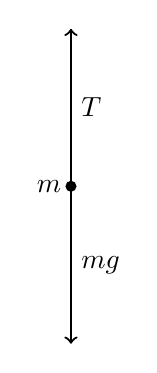
\begin{tikzpicture}
\coordinate (m) at (0,0);
\node[left] at (m) {$m$};
\fill (m) circle [radius=2pt];
\draw[->,thick] (m) -- (0,2) node[midway,right] {$T$};
\draw[->,thick] (m) -- (0,-2) node[midway, right] {$mg$};
\end{tikzpicture}
\caption{} \label{fig:freebody}
\end{wrapfigure}
As the pendulum swings, the tension in the string causes the bob to follow a circular path. At the bottom of the swing the net force on the bob is the combination of the tension in the string and the weight of the object. Therefore we can write our net force equation based off Figure~\ref{fig:freebody} as,
\begin{equation}
F_c=\Sigma F=T-mg=ma,
\end{equation}
where $T$ is the tension in the string, $m$ the mass of the bob, and $F_c$ the centripetal force given by,
\begin{equation} \label{eq:CenForce2}
F_c=\frac{mv^2}{r}.
\end{equation}

\section{Setup I: Spring applied Centripetal Force}
\begin{figure}[h]
\centering
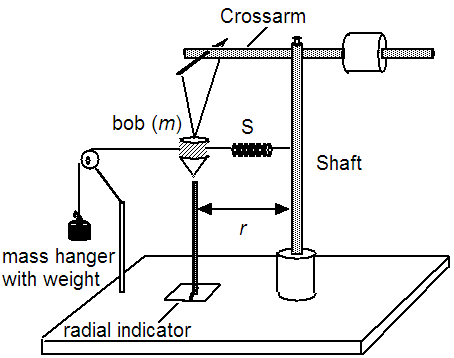
\includegraphics{CenForce_1_Setup} \label{page:CenForce_1_Setup}
\end{figure}

In the experiment apparatus, the centripetal force is applied to the bob (of mass $m$) by a spring, `S,' attached between the mass and the shaft.  The rotation causes the spring to stretch. The force necessary to stretch the spring the same amount can be measured directly using Hooke's Law, which states that the force needed to stretch (or compress) a spring is proportional to the amount, $x,$ the spring is stretched (or compressed),
\[
F_s=-kx,
\]
where k is called the spring constant and is a measurement of the stiffness of the spring.

We will be rotating the mass in a circle of radius $r$ and determining its angular velocity by counting the number of revolutions per second. Using Equation~\eqref{eq:CenForce1} we will calculate the centripetal force $F_c.$ We will also determine the force $F_s$ by attaching a hanging mass to the spring that will stretch to the equivalent distance. The forces $F_c$ and $F_s$ should have equal values within measurement uncertainty.

\subsection*{Procedure}
\begin{enumerate}
\item
Remove the bob (the rotating mass) and determine its mass.
\item
Adjust the radial indicator's position so that it is closest to the shaft.
\item \label{step:CenForce1_start}
Adjust the crossarm at the top of the shaft so that the bob---without the spring attached---hangs over the radial indicator. This is extremely important since when we begin rotating, the string must be vertical so that it only supports the weight of the bob. If the string is not vertical during rotation, the tension in the string would add an unknown horizontal component of force on the bob, and would invalidate our calculations.
\item
Attach the spring between the bob and the shaft.
\item
Attach a mass hanger with a string and hook to the opposite side of the bob.
\item
Add enough mass to the hanger to cause the bob to realign with the radial indicator and record this mass, including the mass of the hanger. The weight of this mass is $F_s.$ This should also be the same force that the spring will apply to the bob under rotation.
\item
As we are making all of our measurements by hand, we will also need to determine the uncertainty of our readings by hand as well. The total uncertainty will be the inherent uncertainty of the masses themselves plus the far greater uncertainty from the sensitivity of the apparatus to changes of mass on the hanger. To determine this, add mass in very small increments (e.g., 1 g increments) and determine the minimum mass necessary to cause a barely noticeable movement of the bob away from the exact alignment with the radial indicator. This uncertainty will not be the same for different masses so we will need to measure it each time we move the radial indicator.
\item
Remove the mass hanger from the string and wrap the string up so that it will be out of the way when we rotate the bob.
\item \label{step:spin_start}
Rotate the shaft until the bob is again lined up with the radial indicator as it moves around in a circle.
\item \label{step:spin_end}
Record the time for 20 revolutions over the radial indicator using a timer. Do this three times and calculate the average and standard deviation of the angular velocity $n.$ The formula for standard deviation can be found on page~\pageref{page:stdDev}.
\item \label{step:Added_Mass}
To test the affect of a greater rotating mass, add 100 g to the bob, then repeat steps~\ref{step:spin_start}--\ref{step:spin_end}.
\item \label{step:CenForce1_end}
Measure the distance $r$ from the center of the shaft to the center of the radial indicator.
\item
Move the radial indicator so that it is midway to its furthest position then repeat steps~\ref{step:CenForce1_start}--\ref{step:CenForce1_end}.
\item
Move the radial indicator to its furthest position from the shaft and repeat steps~\ref{step:CenForce1_start}--\ref{step:CenForce1_end}.
\end{enumerate}

\subsection*{Analysis}
\begin{enumerate}
\item
Calculate the force $F_c$ for all six trials. 
\item
Compare the values of $F_c$ to $F_s$ for the corresponding radius.
\item
Calculate the average of the two forces $F_c$ (for different masses of the bob---see Procedure, step~\ref{step:Added_Mass}) at each radius.
\end{enumerate}

\begin{question}
When the mass of the bob was increased by 100 g and the radius was held constant did the speed vary appropriately? In what way?
\end{question}

\section{Setup II: Centripetal Force on a Pendulum.}
\begin{tabular}{ll}
\begin{minipage}{0.5\textwidth}
For this setup, the Force Sensor will measure the centripetal force on a pendulum bob as it swings back-and-forth. The Photogate will measure the time that the pendulum bob blocks the Photogate beam. We will need to enter the value for the diameter of the pendulum bob. Capstone will calculate and display the speed of the pendulum bob and the centripetal force on the pendulum. We can then use this data to calculate centripetal force based on the measured speed of the pendulum bob. Finally we can compare the calculated and measured values of the centripetal force.
\end{minipage}
&
\begin{minipage}{0.5\textwidth}
\centering
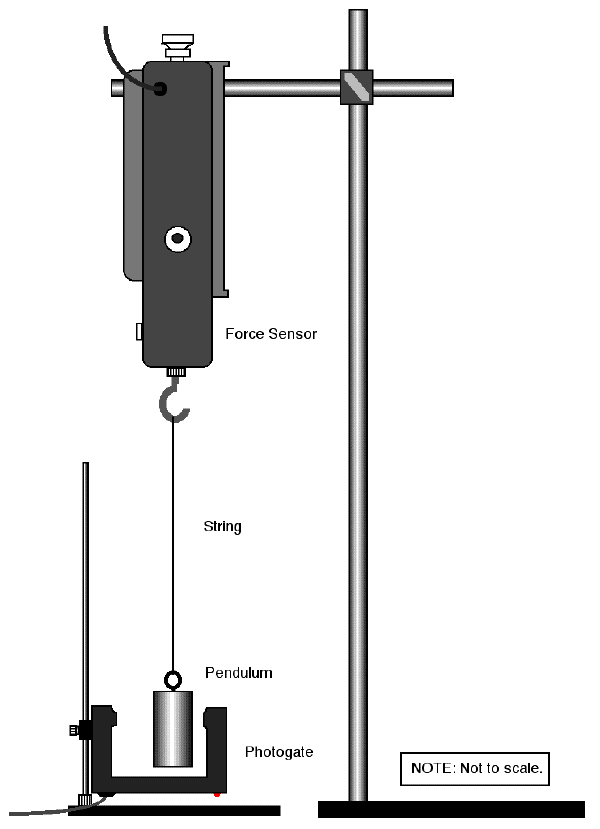
\includegraphics[width=\textwidth]{CenForce_2_Setup}
\end{minipage}
\end{tabular}

\begin{enumerate}
\item
Start Capstone.
\item
Attach a Photogate and a Force Sensor to the 850UI and add the sensors to the appropriate ports in Capstone.
\item
Calibrate the Force Sensor as we did on page~\pageref{page:Calibration}.
\item
We need to set up the Photogate timer for our experiment. Click on the ``Timer Setup" button on the left.
\item
We will be using a Pre-Configured Timer. When Capstone asks us what type of timer we would like to create, select ``One Photogate (Single Flag)."
\item
Check ``Speed" and uncheck all other options.
\item
Measure the diameter of the pendulum bob and enter it in Capstone as the Pendulum Width.
\item
Name the timer as ``Tangential Speed," click Save, and then click ``Timer Setup" to hide the window.
\item
Create a Graph display and add a second plot area to the display 
\includegraphics{Add_New_Plot}
\item
For the upper plot area select ``Force (N)" then select ``Speed (m/s)" for the lower plot area.
\end{enumerate}•

\subsection*{Procedure}
\begin{enumerate}
\item
Measure the mass ($m$) of the bob and record it in the data table.
\item
Use a piece of string that is about one meter long. Tie one end of the string to the Force Sensor hook and the other to the pendulum bob.
\item
Position the Photogate so that the bob blocks the beam when at rest. Adjust the length of the string so that the center of mass of the bob is a the same height as the Photogate's beam.
\item
Measure the length ($r$) of the pendulum from the Force Sensor's hook to the bob's center of mass. Record this length in the data table.
\item
When all the equipment is set up, check the alignment by pull the pendulum bob straight to the side about 15--20 cm. Carefully release the bob so that it swings through the Photogate as smoothly as possible. Adjust the Photogate position as necessary.
\item
Before we begin data collection, press the tare button on the Force Sensor while the pendulum bob is \emph{at rest} and hanging \emph{straight downwards.}
\item
Pull the pendulum bob to the side, click on the Record button and release the bob. Record data for at least 20 seconds then click Stop.
\item
The graph will display plots of the pendulum's centripetal force and tangential velocity. The force plot should be sinusoidal while the velocity plot should be linear. If this is not the case, delete the data run and try again.
\item
\textbf{Print} the graph for each group member.
\end{enumerate}•

\subsection*{Analysis}
\begin{enumerate}
\item \label{step:CenForce2_Analysis_start}
Click on the Force vs Time graph and rescale to fit the data. Click on the Coordinate Tool 
\includegraphics{Coordinates_Tool} and move it to the first or second peak of the plot. Record the value of the centripetal force as shown by the tool.
\item \label{step:CenForce2_Analysis_end}
We want to measure the tangential velocity at the same time at which the force is being measured. Click on the Speed vs Time graph and use the Coordinate Tool to select the data point that occurs at the same time as the data point we have selected in the Force vs Time graph. Record the value of the speed at this data point.
\item
Repeat steps~\ref{step:CenForce2_Analysis_start}--\ref{step:CenForce2_Analysis_end} for four more peaks on the Force vs Time plot.
\item
For each tangential speed value calculate the centripetal force using Equation~\eqref{eq:CenForce2}.
\item
Calculate the percent difference between the measured centripetal force and the calculated centripetal force for each point.
\end{enumerate}•

\begin{question}
Why is it important to tare the Force Sensor before we started data collection for this experiment?
\end{question}
\begin{question}
What are the possible reasons for the differences between the measured and calculated values of centripetal force? Is each possible source of error big or small? Does it have a significant effect on the data?
\end{question}

\begin{samepage}
\hrulefill \\ \\
\emph{Chapter~\ref{chap:Cen_Force}:} \textbf{Centripetal Force}
\begin{enumerate}
\item
\textbf{(1)} Title Page
\item
\textbf{(4)} Purpose
\item
\textbf{(10)} Theory of both setups
\item
\textbf{(5)} Procedure of Setup I
\item
\textbf{(8)} Data Sheet of Setup I
\item
\textbf{(5)} Data Processing Sheet for Setup I. Show sample calculations.
\item
\textbf{(1)} Graph from Setup II
\item
\textbf{(6)} Data Processing Sheet for Setup II. Show sample calculations.
\item
\textbf{(6)} Answer all questions
\item
\textbf{(4)} Conclusion
\end{enumerate}•
\end{samepage}

\newpage
\section{Data Tables}
\subsection*{Setup I}
\subsubsection*{Data Sheet}

{
\doublespacing
\textbf{Be sure to include appropriate units.}\\
Mass of bob\rule[-1mm]{2.5cm}{.1pt}\\
Position 1: $r_1=\rule[-1mm]{2.5cm}{.1pt}$\\
Mass on spring (including hanger) $m_s=\rule[-1mm]{2.5cm}{.1pt}\pm\rule[-1mm]{1.5cm}{.1pt}$\\
\begin{tabular}{@{\hspace{3ex}}p{42em}}
Bob alone. Remember $n_i=20/t_i.$\\
$n_1=\rule[-1mm]{2.5cm}{.1pt}, n_2=\rule[-1mm]{2.5cm}{.1pt}, n_3=\rule[-1mm]{2.5cm}{.1pt}$\\
$n_{average}=\rule[-1mm]{2.5cm}{.1pt}\pm\rule[-1mm]{1.5cm}{.1pt}$\\
Bob + 100 g.\\
$n_1=\rule[-1mm]{2.5cm}{.1pt}, n_2=\rule[-1mm]{2.5cm}{.1pt}, n_3=\rule[-1mm]{2.5cm}{.1pt}$\\
$n_{average}=\rule[-1mm]{2.5cm}{.1pt}\pm\rule[-1mm]{1.5cm}{.1pt}$\\
\end{tabular}
Position 2: $r_2=\rule[-1mm]{2.5cm}{.1pt}$\\
Mass on spring (including hanger) $m_s=\rule[-1mm]{2.5cm}{.1pt}\pm\rule[-1mm]{1.5cm}{.1pt}$\\
\begin{tabular}{@{\hspace{3ex}}p{42em}}
Bob alone.\\
$n_1=\rule[-1mm]{2.5cm}{.1pt}, n_2=\rule[-1mm]{2.5cm}{.1pt}, n_3=\rule[-1mm]{2.5cm}{.1pt}$\\
$n_{average}=\rule[-1mm]{2.5cm}{.1pt}\pm\rule[-1mm]{1.5cm}{.1pt}$\\
Bob + 100 g.\\
$n_1=\rule[-1mm]{2.5cm}{.1pt}, n_2=\rule[-1mm]{2.5cm}{.1pt}, n_3=\rule[-1mm]{2.5cm}{.1pt}$\\
$n_{average}=\rule[-1mm]{2.5cm}{.1pt}\pm\rule[-1mm]{1.5cm}{.1pt}$\\
\end{tabular}
Position 3: $r_3=\rule[-1mm]{2.5cm}{.1pt}$\\
Mass on spring (including hanger) $m_s=\rule[-1mm]{2.5cm}{.1pt}\pm\rule[-1mm]{1.5cm}{.1pt}$\\
\begin{tabular}{@{\hspace{3ex}}p{42em}}
Bob alone.\\
$n_1=\rule[-1mm]{2.5cm}{.1pt}, n_2=\rule[-1mm]{2.5cm}{.1pt}, n_3=\rule[-1mm]{2.5cm}{.1pt}$\\
$n_{average}=\rule[-1mm]{2.5cm}{.1pt}\pm\rule[-1mm]{1.5cm}{.1pt}$\\
Bob + 100 g.\\
$n_1=\rule[-1mm]{2.5cm}{.1pt}, n_2=\rule[-1mm]{2.5cm}{.1pt}, n_3=\rule[-1mm]{2.5cm}{.1pt}$\\
$n_{average}=\rule[-1mm]{2.5cm}{.1pt}\pm\rule[-1mm]{1.5cm}{.1pt}$\\
\end{tabular}
}

\newpage
\subsubsection*{Data Processing}
\begin{doublespace}
\resizebox{0.75\textwidth}{!}{
\begin{tabular}{|l|l@{\hskip 2 cm}|}
\hline
Radius & $F_s (=m_s g)$\\
\hline
$r_1$ &\\
\hline
$r_2$ &\\
\hline
$r_3$ &\\
\hline
\end{tabular}
}\\[8pt]
\resizebox{0.75\textwidth}{!}{
\begin{tabular}{|l|l@{\hskip 2 cm}|}
\hline
Radius & $F_c$ Bob only\\
\hline
$r_1$ &\\
\hline
$r_2$ &\\
\hline
$r_3$ &\\
\hline
\end{tabular}
}\\[8pt]
\resizebox{0.75\textwidth}{!}{
\begin{tabular}{|l|l@{\hskip 2 cm}|}
\hline
Radius & $F_c$ Bob + 100 g\\
\hline
$r_1$ &\\
\hline
$r_2$ &\\
\hline
$r_3$ &\\
\hline
\end{tabular}
}\\[8pt]
\resizebox{0.75\textwidth}{!}{
\begin{tabular}{|l|l|}
\hline
Radius & Average $F_c$ for both masses\\
\hline
$r_1$ &\\
\hline
$r_2$ &\\
\hline
$r_3$ &\\
\hline
\end{tabular}
}
\end{doublespace}

\newpage
\subsection*{Setup II}
\begin{doublespace}
mass of pendulum bob $m=\rule[-1mm]{2.5cm}{.1pt}$ kg\\
length of pendulum $r=\rule[-1mm]{2.5cm}{.1pt}$ m\\ \\
\begin{tabular}{|c|c|c|c|c|}
\hline
Peak & $F_c$ Measured (N) & $v$ (m/s) & $F_c$ Calculated (N) & \% difference\\
\hline
1 &&&&\\
\hline
2 &&&&\\
\hline
3 &&&&\\
\hline
4 &&&&\\
\hline
5 &&&&\\
\hline
\end{tabular}•
\end{doublespace}

\end{document}
